\documentclass[12pt]{article}
\usepackage[utf8]{inputenc}
\usepackage[dvipsnames]{xcolor}
\usepackage[margin=1in]{geometry}
\usepackage{palatino, amsmath, amssymb, amsfonts, hyperref, amsthm, bbm, cancel}
\usepackage[breakable]{tcolorbox}
\usepackage[linesnumbered,lined,boxed,commentsnumbered, ruled]{algorithm2e}
\usepackage{xcolor, graphicx}
\usepackage{xifthen}
\usepackage[shortlabels]{enumitem}
\usepackage[parfill]{parskip}
\usepackage{hyperref}
\usepackage[cal=pxtx]{mathalfa}
\usepackage{fancyhdr} 
\usepackage{url}
\setlength\parindent{0pt}
\usepackage{tikz}
\usetikzlibrary{positioning}
\hypersetup{
    colorlinks=true,
    linkcolor=blue,
    filecolor=magenta,      
    urlcolor=cyan,
}
\newcommand{\pink}[1]{{\color{Magenta} #1}}
\newcommand{\gray}[1]{{\color{Gray} #1}}
\newcommand{\red}[1]{{\color{red} #1}}
\newcommand{\todo}[1]{{\color{red} TODO: #1}}
\renewcommand{\comment}[1]{{\color{Blue} Comment:  #1}}
\newcommand{\inabox}[1]{\begin{tcolorbox}[parbox=false, colback=White, breakable] #1 \end{tcolorbox}}

\newcommand{\R}{\mathbb{R}}
\newcommand{\N}{\mathbb{N}}
\newcommand{\p}{\mathbb{P}}
\renewcommand{\subset}{\subseteq}

\pagestyle{fancyplain}
\lhead{\fancyplain{}{Blair Yang, Murphy Tian, Tony Chen}}
% Right side of header. First page empty (as above).
\rhead{\fancyplain{}{CSC311 Final Project Report}}
\setlist[enumerate,1]{a.)} % Level 1, 2 enumerate styles
\setlist[enumerate,2]{i.)}
%\setlist[itemize,1]{$\cdot$} % Small dot

\newcommand{\SOLUTION}{}
\newcommand{\solution}[1]{
    \ifdefined\SOLUTION
        \newpage
        \textbf{#1.} 
    \else
    \fi
}

\newcommand{\handout}[1]{
    \ifdefined\SOLUTION
        #1
    \else
    \fi
}
\newtheorem{theorem}{Theorem}


% Counter for Questions
\newcounter{question}

% Question
\newcommand{\question}[2]{%
	\stepcounter{question}
	\vspace{.25in} \textbf{Q\arabic{question} 
		\ifthenelse{\isempty{#1}}%
		{}% if no points
		{[#1 Points]\ }% if #1 is not empty
		#2}\vspace{0.10in}
}

% Subquestion
\newcommand{\qpart}[2]{%
	\vspace{.10in} \textbf{(#1)}
	\ifthenelse{\isempty{#2}}%
	{}% if no points
	{[#2 Points]}% if #1 is not empty
}

\newcommand{\references}{\vspace{.25in}\textbf{References}\vspace{.10in}}

% Solution to question
\newcommand{\sol}{\vspace{.25in}\textbf{Solution}\vspace{.10in}}

% Solution to subquestion
\newcommand{\solpart}[1] {\vspace{.10in}\textbf{(#1)}}

% Should the solutions be displayed?
\newif\ifsolutions
\solutionstrue

% Should the marking scheme be displayed?
\newif\ifmarkingscheme
\markingschemefalse

% Math commands
\newcommand{\set}[1]{\{#1\}}
\newcommand{\floor}[1]{\lfloor#1\rfloor}
\newcommand{\ceil}[1]{\lceil#1\rceil}
\DeclareMathOperator*{\argmin}{arg\,min}
\DeclareMathOperator*{\argmax}{arg\,max}

\usepackage[linesnumbered,lined,boxed,commentsnumbered, ruled]{algorithm2e}
\usepackage{algorithm2e}

\title{CSC 311 Final Project Report}
\author{Blair Yang, Murphy Tian, Tony Chen} % TODO PUT NAMES HERE
\date{Due: Mar 30, 2023 at 5:00pm} % TODO PUT DATE HERE
\begin{document}
\maketitle
\newpage
\section*{Part A}
\subsection*{k-Nearest Neightbor}
In this problem, using the provided code, you will experiment with k-Nearest Neighbor(kNN) algorithm.

The provided kNN code performs collaborative filtering that uses other students' answers to predict whether the specific student can correctly answer some diagnostic questions. In particular, the starter code implements user-based collaborative filtering: given a user, kNN finds the closest user that similarly answered other questions and predicts the correctness based on the closest students' correctness. The core underlying assumption is that if student A has the same correct and incorrect answers on other diagnostic questions as student B, A's correctness on specific diagnostic questions matches that of student B.
\begin{itemize}
	\item [(a)] Complete a function \textbf{main} located at \textbf{knn.py} that runs KNN for different values of $k \in \{1, 6, 11, 16, 21, 26\}$ Plot and report the accuracy on the validation data as a function of k.
	\begin{center}
		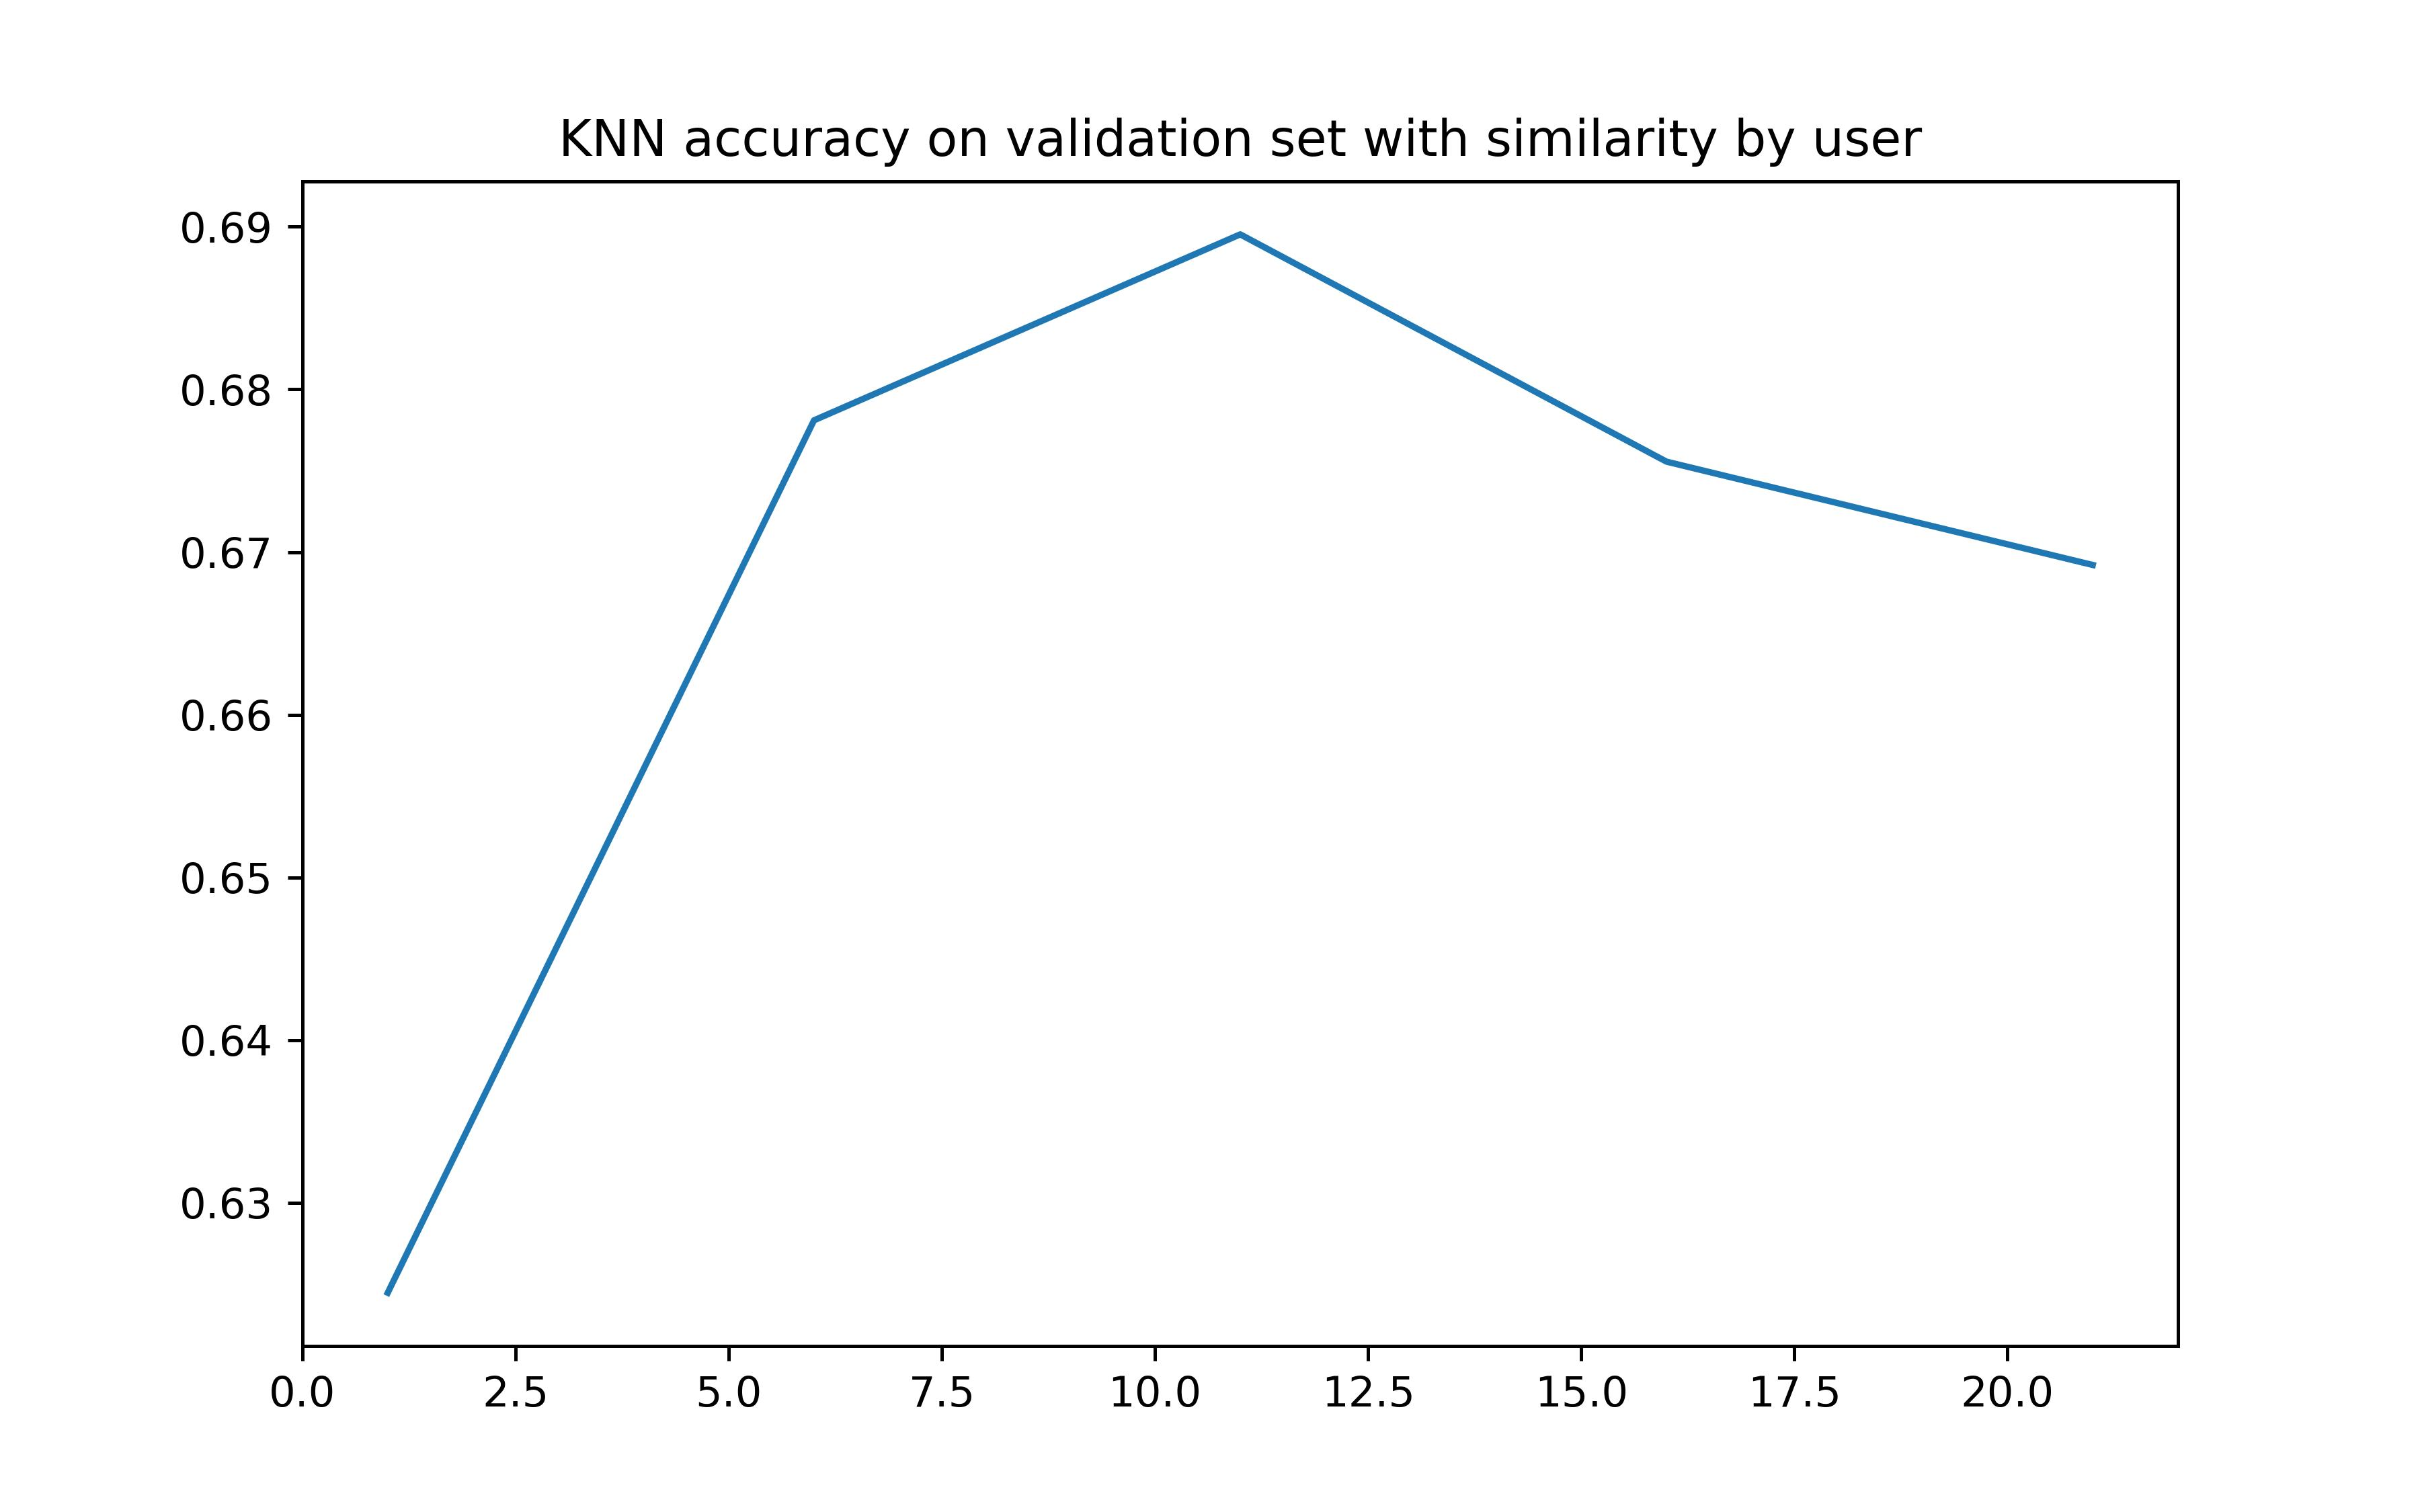
\includegraphics[scale=0.8]{../out/KNN_user.jpg}
	\end{center}
	\begin{align*}
		\text{Validation Accuracy} \mid_{k=1} &:= 0.6244707874682472\\
		\text{Validation Accuracy} \mid_{k=6} &:=0.6780976573525261 \\
		\text{Validation Accuracy} \mid_{k=11} &:= 0.6895286480383855\\
		\text{Validation Accuracy} \mid_{k=16} &:=0.6755574372001129 \\
		\text{Validation Accuracy} \mid_{k=21} &:= 0.6692068868190799\\
		\text{Validation Accuracy} \mid_{k=26} &:= 0.6522720858029918
	\end{align*}

	\item [(b)] Choose $k^*$ that has the highest performance on validation data. Report the chosen $k^*$ and the final test accuracy.
	
	Test accuracy with maximum valid accuracy with $k^* = 11$ is 0.6841659610499576
	\item[(c)] Implement a function performs item-based collaborative filtering instead of user-based collaborative filtering. Given a question, kNN finds the closest question's correctness. State the underlying assumption on item-based collaborative filtering. Repeat part (a) and (b) with item-based collaborative filtering.
	\begin{center}
		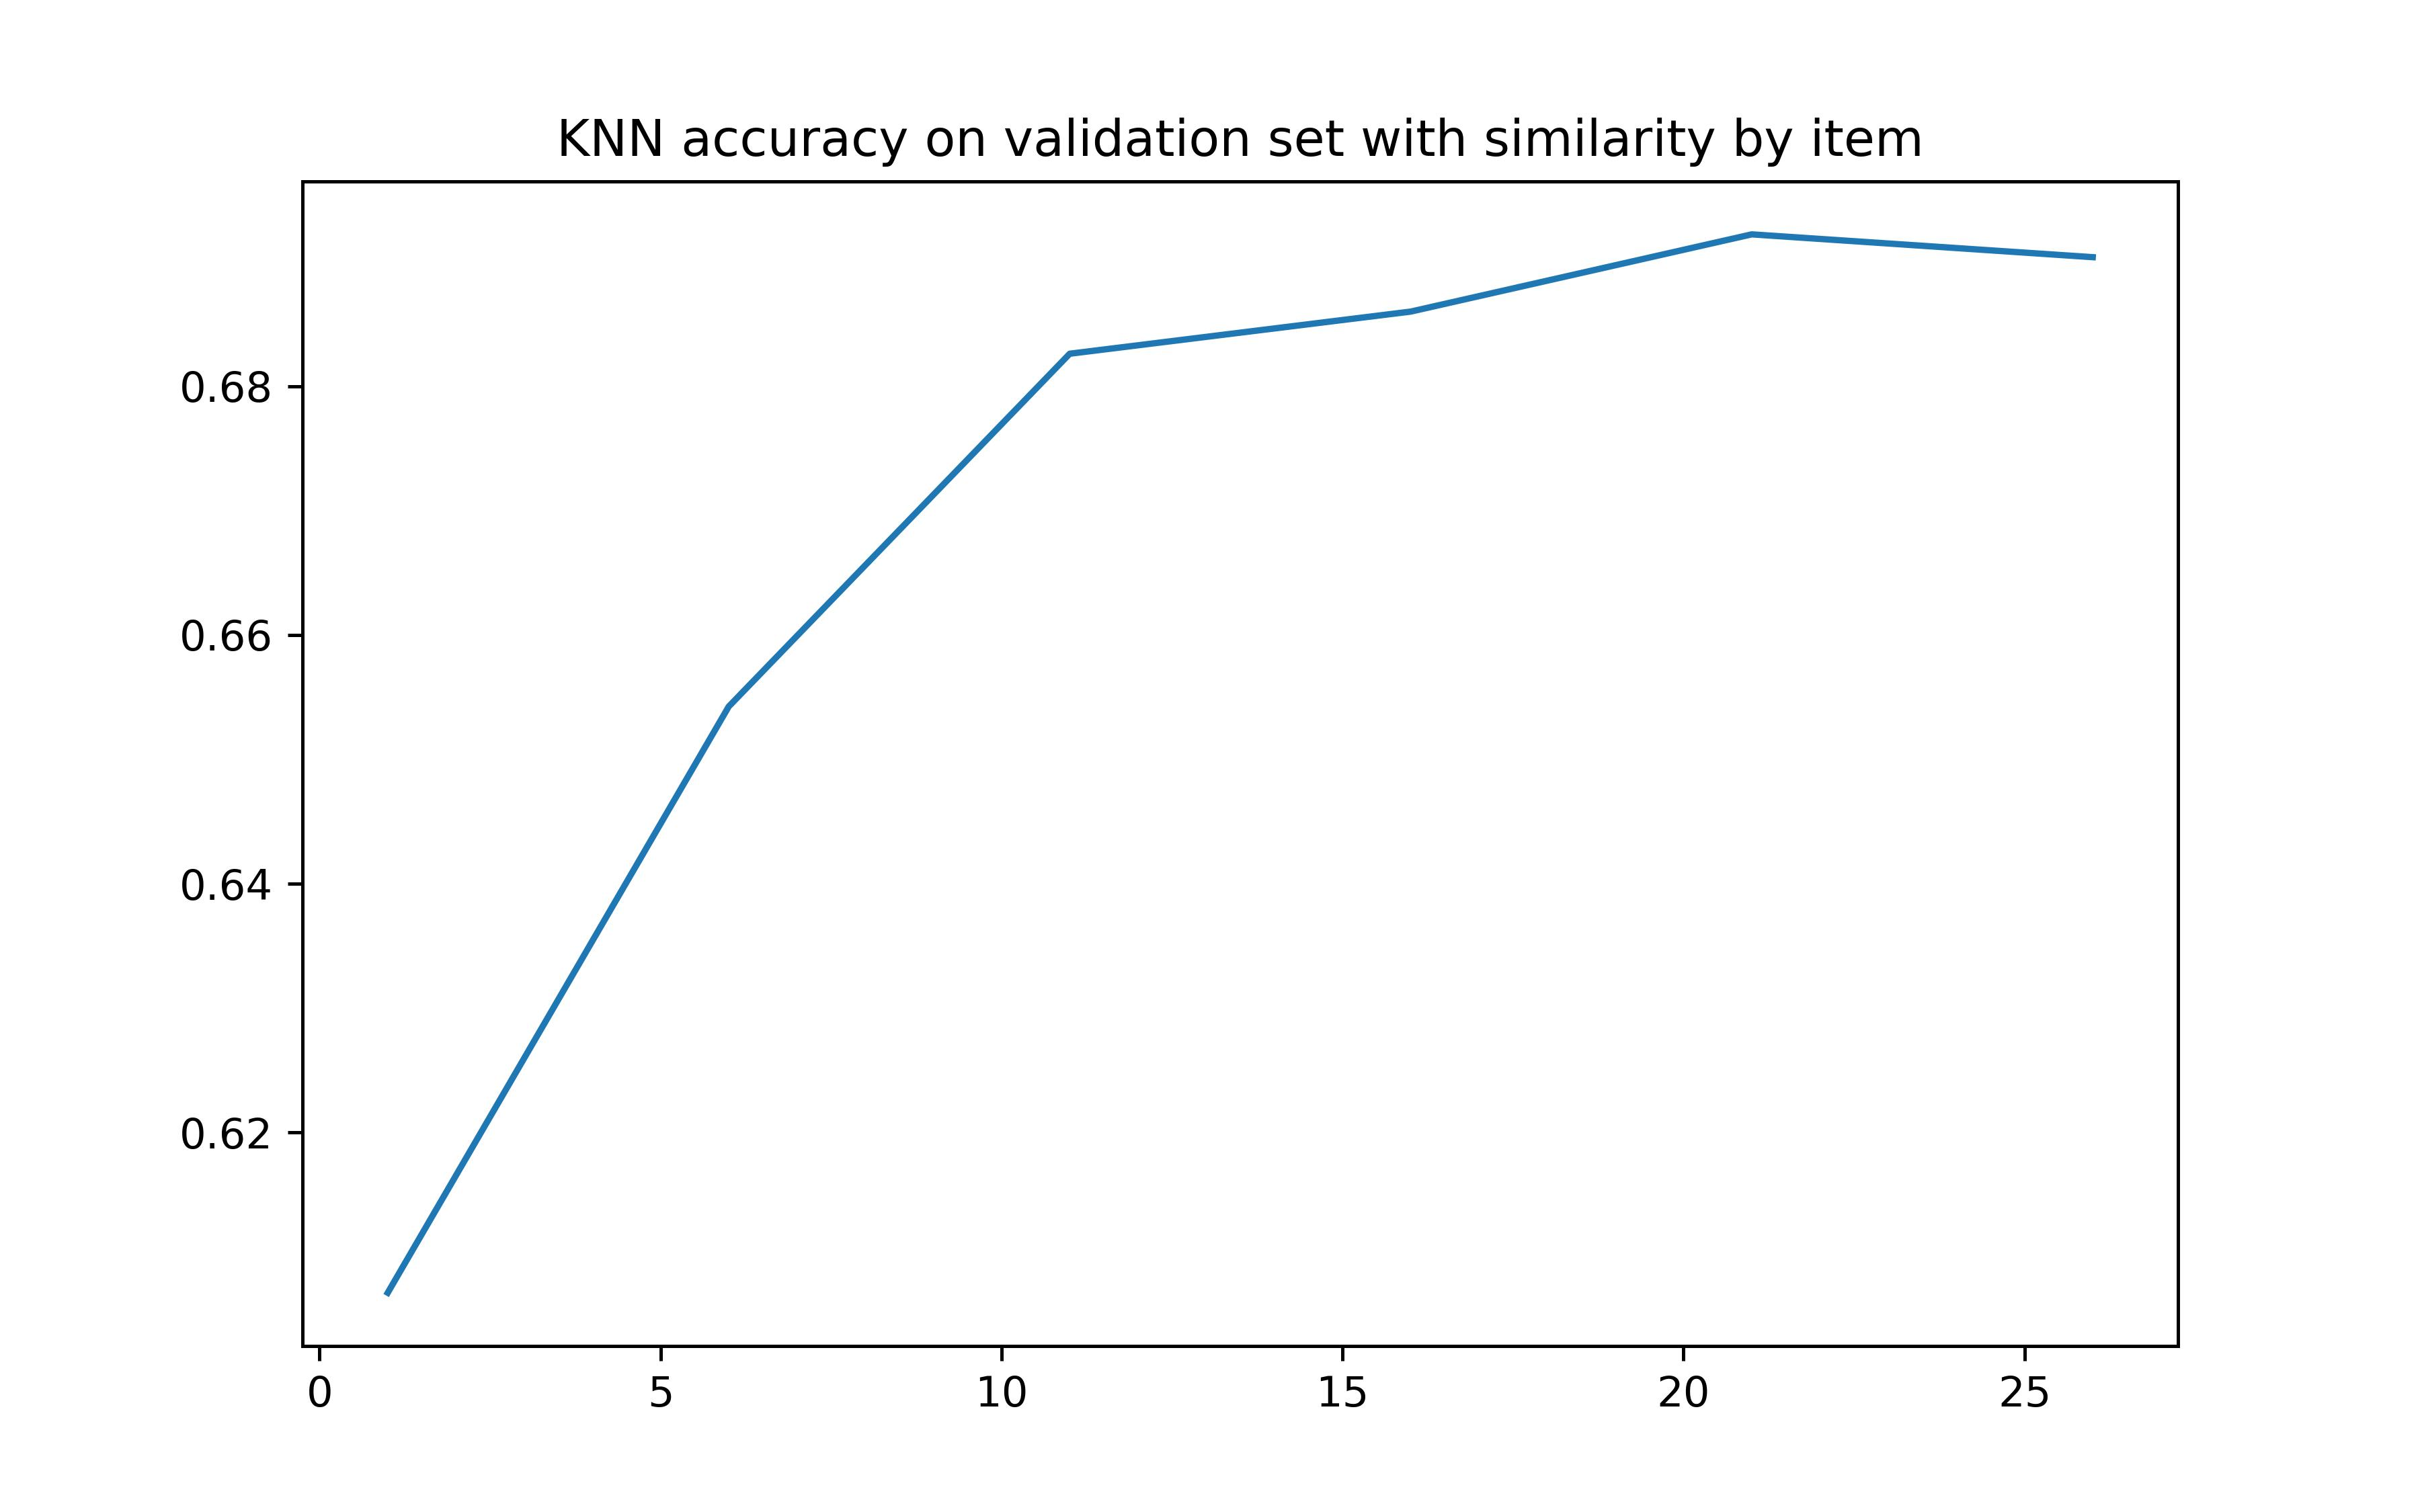
\includegraphics[scale=0.8]{../out/KNN_item.jpg}
	\end{center}
	\begin{align*}
		\text{Validation Accuracy} \mid_{k=1} &:= 0.607112616426757\\
		\text{Validation Accuracy} \mid_{k=6} &:= 0.6542478125882021\\
		\text{Validation Accuracy} \mid_{k=11} &:= 0.6826136042901496\\
		\text{Validation Accuracy} \mid_{k=16} &:= 0.6860005644933672\\
		\text{Validation Accuracy} \mid_{k=21} &:= 0.6922099915325995\\
		\text{Validation Accuracy} \mid_{k=26} &:= 0.69037538808919
	\end{align*}
	Test accuracy with maximum valid accuracy with k* = 21 is 0.6816257408975445.
	
	\item [(d)] Compare the test performance between user- and item- based collaborative filtering. State which method performs better.
	\begin{center}
		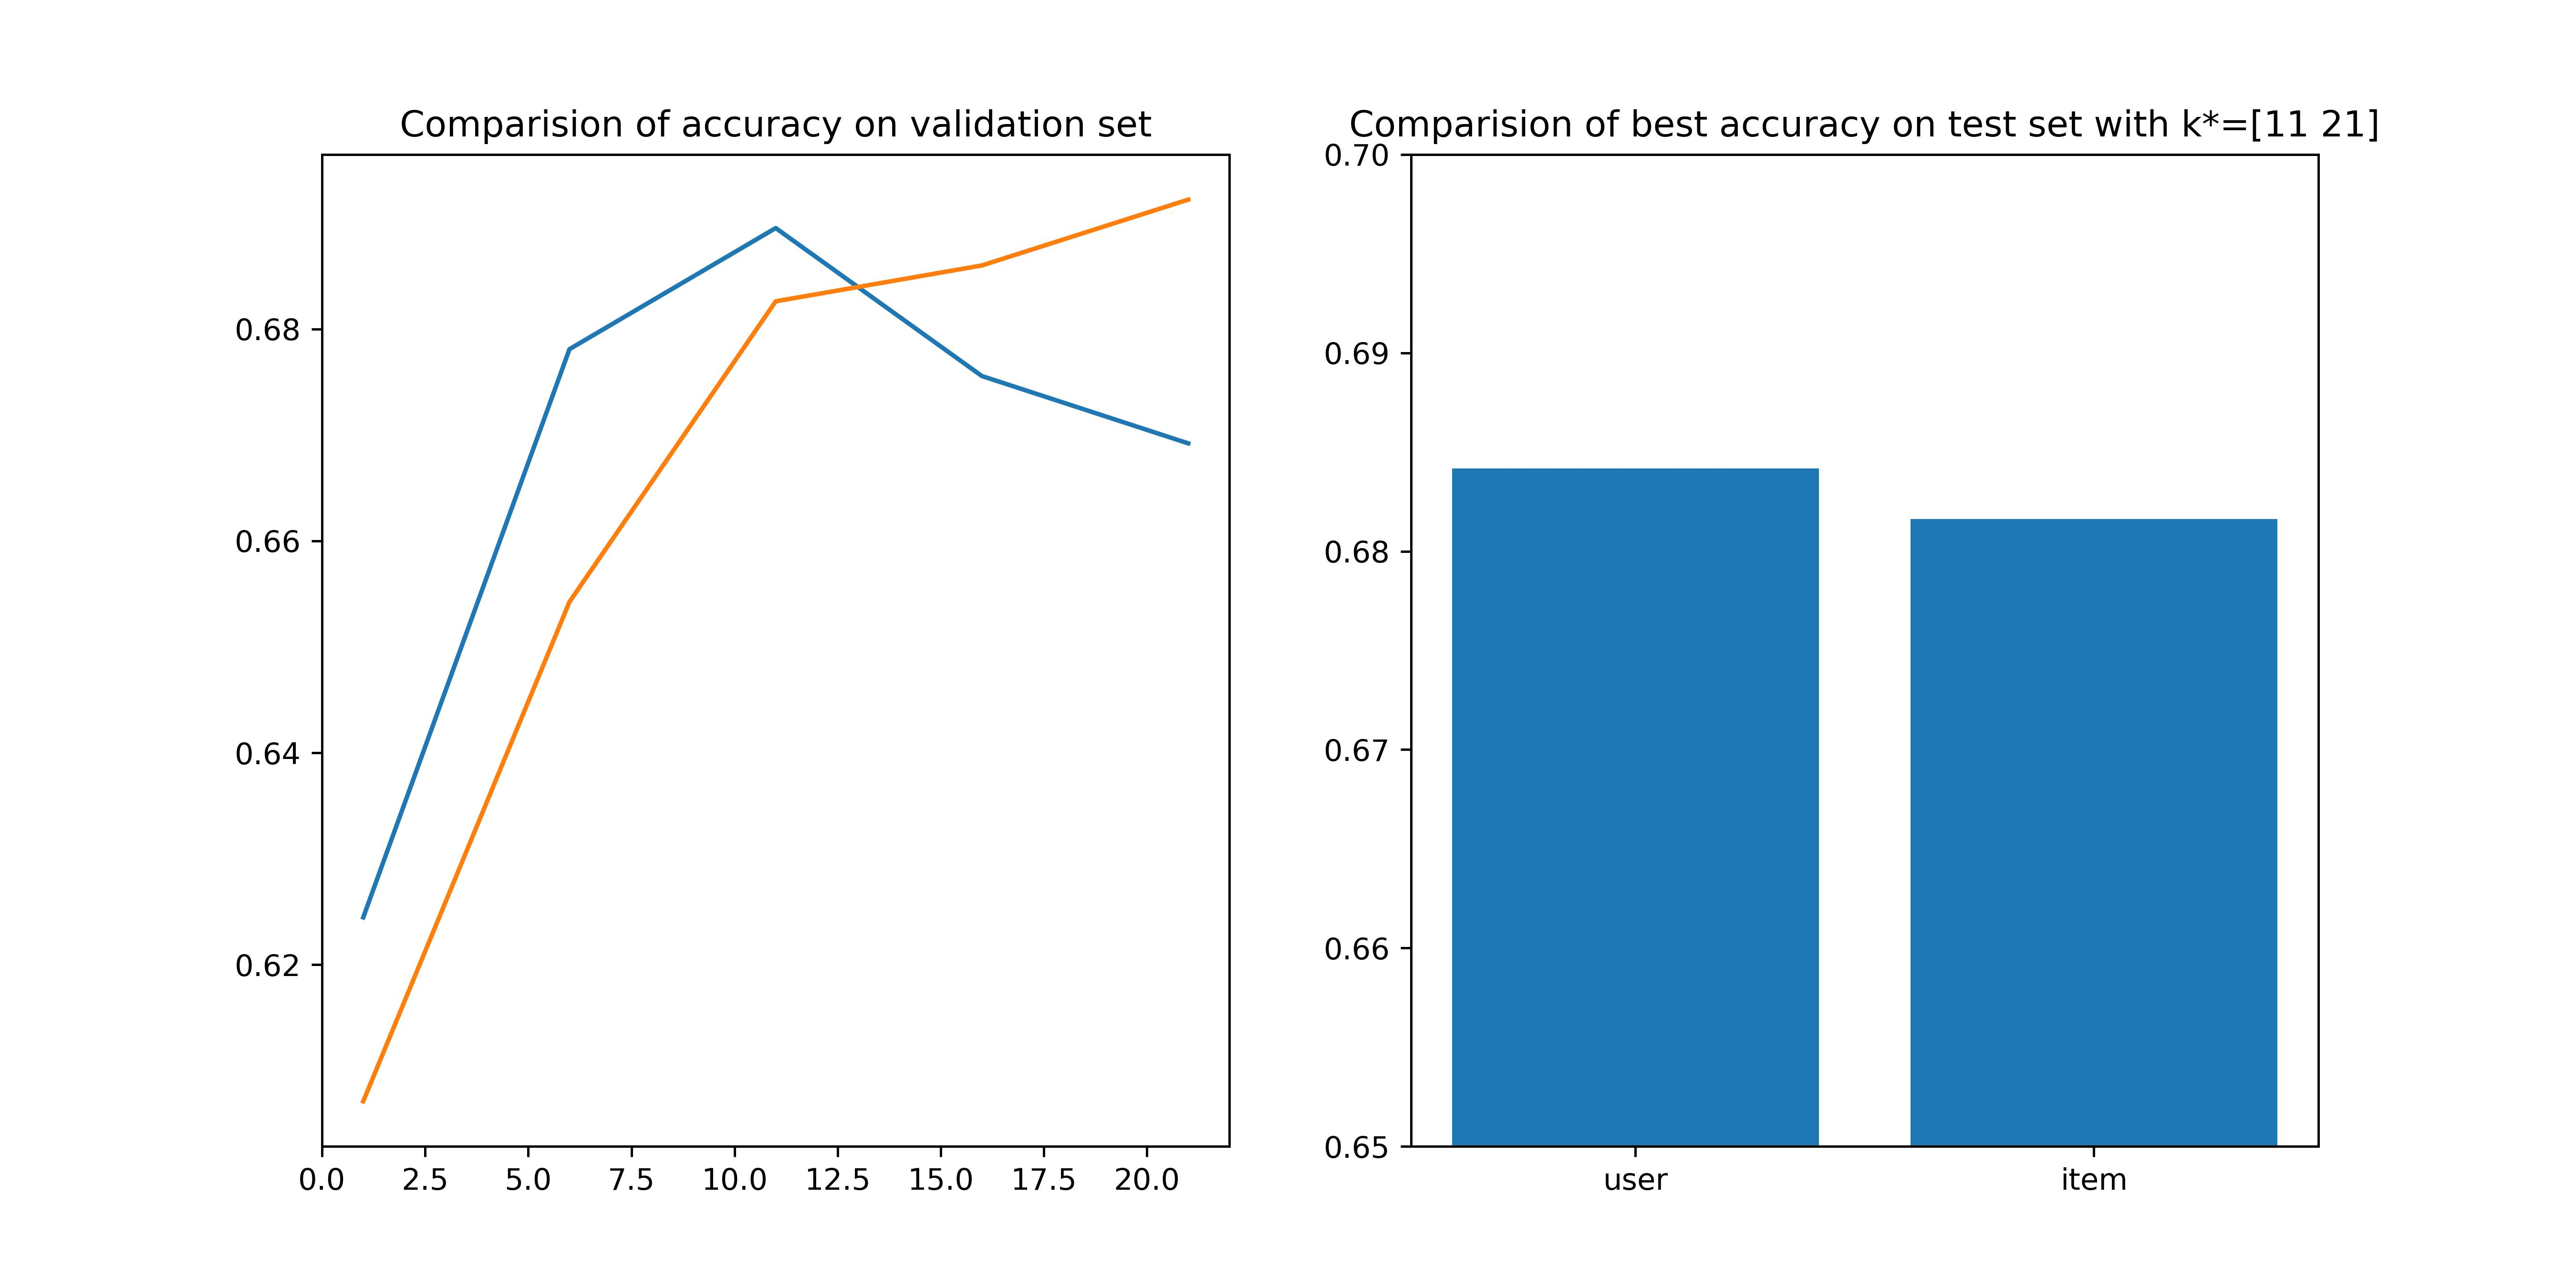
\includegraphics[scale=0.6]{../out/KNN_compare.jpg}
	\end{center}
	Based on the figure above, we claim them the user- collaborative filtering have better performance.
		\item [(e)] List at least two potential limitations of kNN for the task you are given.
		
		The curse of Dimensionality; bid computation cost on the test set.	
\end{itemize}
\newpage
\subsection*{Item Response Theory}
In this problem, you will implement an Item-Response Theory (IRT) model to predict students' correctness to diagnostic questions.

The IRT assigns each student an ability value and each question a difficulty value to formulate a probability distribution> In the one-parameter IRT model, $\beta_j$ represents the difficulty of the question j, and $\theta_i$ that represents the i-th students ability. Then, the probability that the question j is correctly answered by student i is formulated as:
\begin{equation*}
	p(c_{ij} = 1 | \theta_{i}, \beta_{j}) = \frac{exp(\theta_i - \beta_j)}{1 + exp(\theta_i -\beta_j)}
\end{equation*}
\begin{enumerate}
	\item Derive the log-likelihood $\logp(C|\theta, \beta)$ for all students and questions. Here \textbf{C} is the sparse matrix. Also, show the derivative of the log-likelihood with respect $\theta_i$ and $\beta_j$\\(Hint: recall the derivative of the logistic model with respect to the parameters.) 
\inabox{From the given equation, we know that $c_{ij}=1$ if the student answers correctly, and $c_{ij}=0$ if the student answers incorrectly.\\
	Hence, we claim the probability that
$$p(c_{ij} | \theta_i, \beta_j) = (\frac{exp(\theta_i -\beta_j)}{1 + exp(\theta_i -\beta_j)})^{c_{ij}}(\frac{1}{1 + exp(\theta_i -\beta_j)})^{(1 - c_{ij})}$$
Assume the responses from students being independently and identically distributed, thus, the joint probability is the product of the individual probabilities:
\begin{align*}
	\log_p (C| \theta, \beta) &= \sum_i \sum_j c_{ij} \log \frac{exp(\theta_i - \beta_j)}{1 + exp(\theta_i -\beta_j)} + (1 - c_{ij}) \log \frac{exp(\theta_i - \beta_j)}{1 + exp(\theta_i -\beta_j)}\\
&= \sum_i\sum_j c_{ij}(\theta_i -\beta_j) - \log (1 + exp(\theta_i -\beta_j))
\end{align*}
Then, taking the derivative of the logistic model with respect to $\theta_i, \beta_j$, we have
\begin{align*}
	\frac{\partial \log p (C | \theta, \beta)}{\partial \theta_i} &= \sum_j c_{ij} - \frac{exp(\theta_i - \beta_j)}{1 + exp(\theta_i -\beta_j)} \\
	\frac{\partial \log p (C | \theta, \beta)}{\partial \beta_j} &= - \sum_i c_{ij} + \frac{exp(\theta_i - \beta_j)}{1 + exp(\theta_i -\beta_j)}
\end{align*}}
	\item Implement missing functions that performs alternating gradient descent on $\theta$ and $\beta$ to maximize the log-likelihood. Report the hyperparameters you selected. With your chosen hyperparameters, report the training curve that shows the training and validation log-likelihoods as a function of iteration.
	\inabox{Taking hyperparameter that learning rate = 0.01, iterations = 20}
	\end{enumerate}
	\begin{center}
			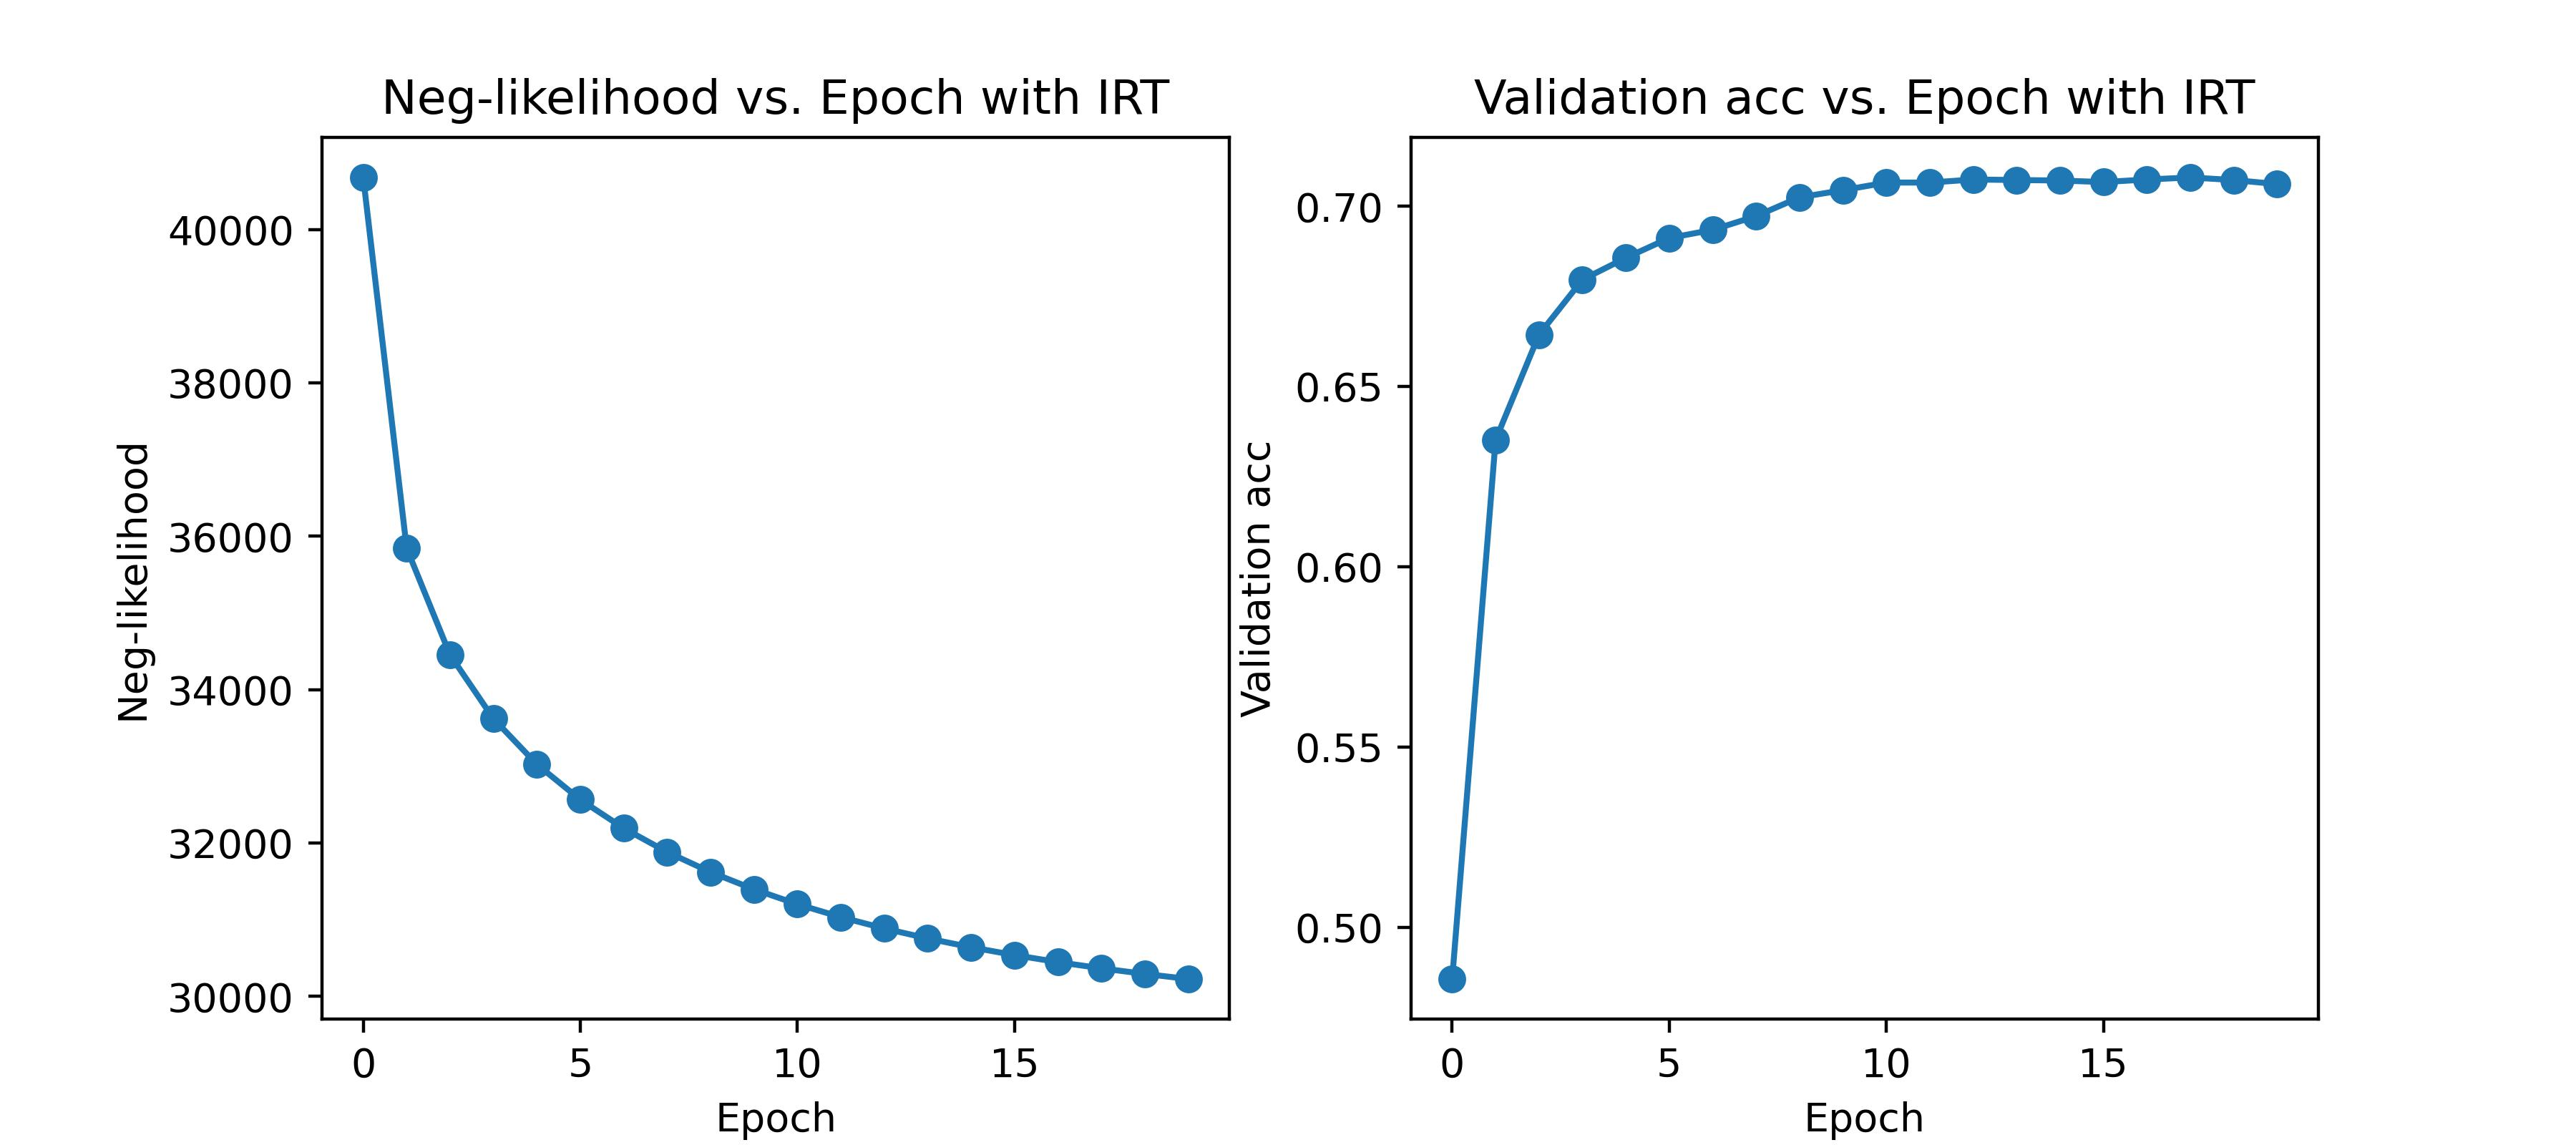
\includegraphics[scale=0.5]{../out/irt.jpg}
	\end{center}
	\begin{enumerate}
	\item [c.)] With the implemented code, report the final validation and test accuracies.
	\inabox{the final validation := 0.709991532599492\\
	final test accuracy := }
	\item [d.)]Select three questions $j_1, j_2$, and $j_3$. Using the trained $\theta$ and $\beta$, plot three curves on the same plot that shows the probability of the correct response $p(c_{ij} = 1)$ as a function of $\theta$ given a question j. Comment on the shape of the curves  and briefly describe what these curves represent.
\end{enumerate}

\end{document}